\documentclass[12pt,]{article}
\usepackage{lmodern}
\usepackage{amssymb,amsmath}
\usepackage{ifxetex,ifluatex}
\usepackage{fixltx2e} % provides \textsubscript
\ifnum 0\ifxetex 1\fi\ifluatex 1\fi=0 % if pdftex
  \usepackage[T1]{fontenc}
  \usepackage[utf8]{inputenc}
\else % if luatex or xelatex
  \ifxetex
    \usepackage{mathspec}
  \else
    \usepackage{fontspec}
  \fi
  \defaultfontfeatures{Ligatures=TeX,Scale=MatchLowercase}
    \setmainfont[]{Times New Roman}
\fi
% use upquote if available, for straight quotes in verbatim environments
\IfFileExists{upquote.sty}{\usepackage{upquote}}{}
% use microtype if available
\IfFileExists{microtype.sty}{%
\usepackage{microtype}
\UseMicrotypeSet[protrusion]{basicmath} % disable protrusion for tt fonts
}{}
\usepackage[margin=2.54cm]{geometry}
\usepackage{hyperref}
\hypersetup{unicode=true,
            pdftitle={Examining the Hydrologic Properties of the Missouri River Basin},
            pdfauthor={Rachel Bash, Keqi He, Caroline Watson, and Haoyu Zhang},
            pdfborder={0 0 0},
            breaklinks=true}
\urlstyle{same}  % don't use monospace font for urls
\usepackage{graphicx,grffile}
\makeatletter
\def\maxwidth{\ifdim\Gin@nat@width>\linewidth\linewidth\else\Gin@nat@width\fi}
\def\maxheight{\ifdim\Gin@nat@height>\textheight\textheight\else\Gin@nat@height\fi}
\makeatother
% Scale images if necessary, so that they will not overflow the page
% margins by default, and it is still possible to overwrite the defaults
% using explicit options in \includegraphics[width, height, ...]{}
\setkeys{Gin}{width=\maxwidth,height=\maxheight,keepaspectratio}
\IfFileExists{parskip.sty}{%
\usepackage{parskip}
}{% else
\setlength{\parindent}{0pt}
\setlength{\parskip}{6pt plus 2pt minus 1pt}
}
\setlength{\emergencystretch}{3em}  % prevent overfull lines
\providecommand{\tightlist}{%
  \setlength{\itemsep}{0pt}\setlength{\parskip}{0pt}}
\setcounter{secnumdepth}{5}
% Redefines (sub)paragraphs to behave more like sections
\ifx\paragraph\undefined\else
\let\oldparagraph\paragraph
\renewcommand{\paragraph}[1]{\oldparagraph{#1}\mbox{}}
\fi
\ifx\subparagraph\undefined\else
\let\oldsubparagraph\subparagraph
\renewcommand{\subparagraph}[1]{\oldsubparagraph{#1}\mbox{}}
\fi

%%% Use protect on footnotes to avoid problems with footnotes in titles
\let\rmarkdownfootnote\footnote%
\def\footnote{\protect\rmarkdownfootnote}

%%% Change title format to be more compact
\usepackage{titling}

% Create subtitle command for use in maketitle
\providecommand{\subtitle}[1]{
  \posttitle{
    \begin{center}\large#1\end{center}
    }
}

\setlength{\droptitle}{-2em}

  \title{Examining the Hydrologic Properties of the Missouri River Basin}
    \pretitle{\vspace{\droptitle}\centering\huge}
  \posttitle{\par}
  \subtitle{\url{https://github.com/cwatson1013/Hydrologic_Data_Analysis_Final_Proj}}
  \author{Rachel Bash, Keqi He, Caroline Watson, and Haoyu Zhang}
    \preauthor{\centering\large\emph}
  \postauthor{\par}
    \date{}
    \predate{}\postdate{}
  

\begin{document}
\maketitle
\begin{abstract}
The Missouri River provides critical water resources that drives the
region's agriculture, industry, and ecosystems. This is a region that
experiences surface water variability, characterized by damaging floods
and severe droughts, greatly impacting the agricultural production of
the area. This project highlights the changes in streamflow and water
quality over time, and identifies key characteristics of the
river\ldots{}.Twenty six sites across the lower Missouri River Basin
were examined in order to get a fuller picture of the Missouri River and
its tributaries over time.
\end{abstract}

\textless{}Information in these brackets are used for annotating the
RMarkdown file. They will not appear in the final version of the PDF
document\textgreater{}

\newpage
\tableofcontents 
\newpage
\listoftables 
\newpage
\listoffigures 
\newpage

\textless{}Note: set up autoreferencing for figures and tables in your
document\textgreater{}

\hypertarget{research-question-and-rationale}{%
\section{Research Question and
Rationale}\label{research-question-and-rationale}}

\textless{}Paragraph detailing the rationale for your analysis. What is
the significant application and/or interest in this topic? Connect to
environmental topic(s)/challenge(s).\textgreater{}

\textless{}Paragraph detailing your research question(s) and goals. What
do you want to find out? Include a sentence (or a few) on the dataset
you are using to answer this question - just enough to give your reader
an idea of where you are going with the analysis.\textgreater{}

\newpage

\hypertarget{dataset-information}{%
\section{Dataset Information}\label{dataset-information}}

\textless{}Information on how the dataset for this analysis were
collected, the data contained in the dataset, and any important pieces
of information that are relevant to your analyses. This section should
contain much of same information as the README file for the dataset but
formatted in a way that is more narrative.\textgreater{}

\textless{}Add a table that summarizes your data structure. This table
can be made in markdown text or inserted as a \texttt{kable} function in
an R chunk. If the latter, do not include the code used to generate your
table.\textgreater{}

\textless{}C will do data table for water quality and daily values, R
will do for high freq\textgreater{}

\newpage

\hypertarget{exploratory-data-analysis-and-wrangling}{%
\section{Exploratory Data Analysis and
Wrangling}\label{exploratory-data-analysis-and-wrangling}}

\textless{}Include R chunks for 5+ lines of summary code (display code
and output), 3+ exploratory graphs (display graphs only), and any
wrangling you do to your dataset(s).\textgreater{}

\textless{}Include text sections to accompany these R chunks to explain
the reasoning behind your workflow, and the rationale for your
approach.\textgreater{}

\newpage

\hypertarget{analysis}{%
\section{Analysis}\label{analysis}}

\textless{}Include R chunks for 3+ statistical tests (display code and
output) and 3+ final visualization graphs (display graphs
only).\textgreater{}

\textless{}Include text sections to accompany these R chunks to explain
the reasoning behind your workflow, rationale for your approach, and the
justification of meeting or failing to meet assumptions of
tests.\textgreater{}

\newpage

\hypertarget{summary-and-conclusions}{%
\section{Summary and Conclusions}\label{summary-and-conclusions}}

\textless{}Summarize your major findings from your analyses. What
conclusions do you draw from your findings? Make sure to apply this to a
broader application for the research question you have
answered.\textgreater{}

\hypertarget{example-for-autoreferencing}{%
\subsection{Example for
autoreferencing}\label{example-for-autoreferencing}}

As seen by \autoref{fig:foo}, Absorbance values are not normally
distributed. This is expected, as we are dealing with ecological data.

\begin{figure}
\centering
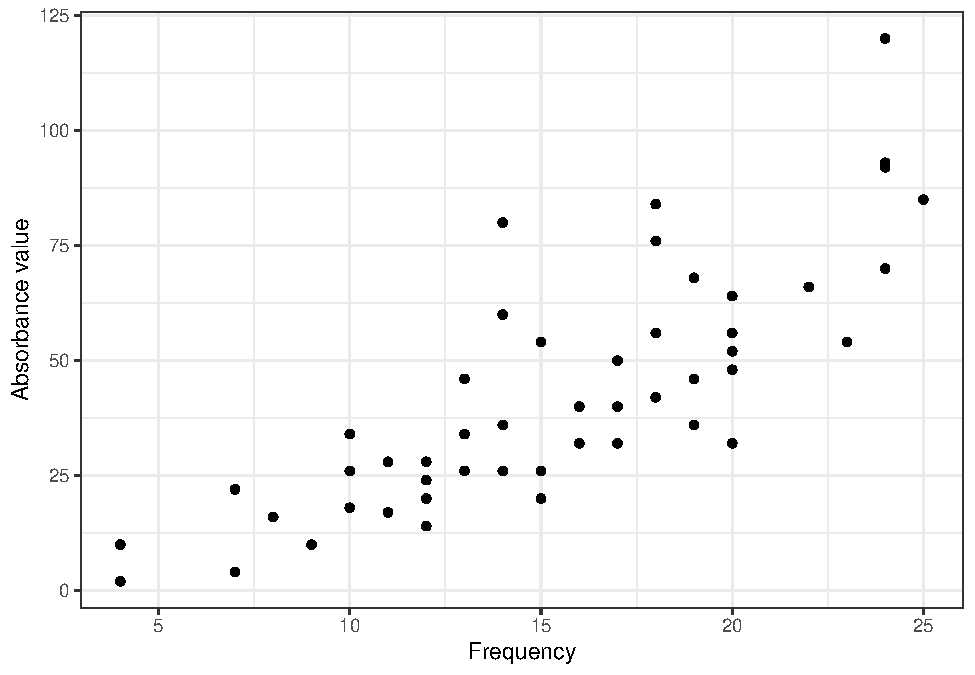
\includegraphics{Project_Template_files/figure-latex/foo-1.pdf}
\caption{\label{fig:foo}Absorbance frequency}
\end{figure}


\end{document}
